\documentclass{report}
\usepackage[a4paper, left=1.5cm, right=1.5cm, top=1cm, bottom=1cm]{geometry}
\usepackage{tikz,tcolorbox}
\usepackage{amsmath}
\usepackage[table,xcdraw]{xcolor}
\usepackage{listings}
\usepackage{array,multirow} % For customizing tables
\usepackage{booktabs} % For better horizontal lines
\usepackage{makecell}
\setlength{\parindent}{0pt}

\lstset{
    language=SQL,                    % Set language to SQL
    basicstyle=\ttfamily\small,      % Font size and family for code
    keywordstyle=\color{blue}\bfseries, % Color for SQL keywords
    commentstyle=\color{gray},       % Color for comments
    stringstyle=\color{red},         % Color for strings
    numbers=left,                    % Show line numbers on the left
    numberstyle=\tiny\color{gray},   % Line number font and color
    stepnumber=1,                    % Line number step
    breaklines=true,                 % Wrap long lines
    frame=single,                    % Add a frame around code
    tabsize=2,                       % Set tab size
    showstringspaces=false           % Hide spaces in strings
}

\definecolor{commentgray}{HTML}{676160}
\definecolor{messagegreen}{HTML}{17B867}
\definecolor{myblue}{HTML}{10C2C4}

\tcbuselibrary{skins, breakable, theorems}


\newtcolorbox{prettyBox}[2]{
  enhanced,
  colback=white!90!#2,   % Background color based on the second parameter (color)
  colframe=#2!60!black,  % Frame color based on the second parameter (color)
  coltitle=white,        % Title color (white)
  fonttitle=\bfseries\Large,
  title=#1,              % Title from the first parameter
  boxrule=1mm,
  arc=0.5mm,
  drop shadow=#2!35!gray, % Drop shadow color based on the second parameter (color)
}

\setcellgapes{2pt}  % Adjust padding as needed
\makegapedcells
\usepackage{titlesec}

\usepackage{forest}

\titleformat{\chapter}[display]
    {\normalfont\huge\bfseries}{\chaptertitlename\ \thechapter}{20pt}{\Huge}
\titlespacing*{\chapter}{0pt}{0pt}{15pt}

\titleformat{\chapter}[hang]
  {\normalfont\huge\bfseries}
  {\thechapter\quad}
  {0pt}
  {}

\begin{document}

\renewcommand{\arrayrulewidth}{0.75mm} % Set line thickness
\setlength{\tabcolsep}{10pt} % Set horizontal padding
\renewcommand{\arraystretch}{1} % Set vertical padding (1.0 is default)
\arrayrulecolor{myblue!70!black}

\usetikzlibrary{positioning}


\chapter{Introduction}

\section{Scalability}

\begin{tikzpicture}[remember picture, overlay]
\node[
    fill=myblue!40!white,
    rounded corners=4pt,
    text=myblue!25!black,
    minimum height=0.5cm,
    minimum width=1cm
]
at ([yshift=9.65cm,xshift=9cm]current page.center)
{ };

\node[
    fill=myblue!40!white,
    rounded corners=4pt,
    text=myblue!25!black,
    minimum height=0.5cm,
    minimum width=1.5cm
]
at ([yshift=10.4cm,xshift=9cm]current page.center)
{ };

\node[
    fill=myblue!40!white,
    rounded corners=4pt,
    text=myblue!25!black,
    minimum height=0.5cm,
    minimum width=2cm
]
at ([yshift=11.15cm,xshift=9cm]current page.center)
{ };
\end{tikzpicture}




\begin{tikzpicture}[remember picture, overlay]


\node[
    fill=myblue!40!white,
    rounded corners=4pt,
    text=myblue!25!black,
    minimum height=0.5cm,
    minimum width=0.75cm
]
at ([yshift=7.75cm,xshift=7cm]current page.center)
{ };


\node[
    fill=myblue!40!white,
    rounded corners=4pt,
    text=myblue!25!black,
    minimum height=0.5cm,
    minimum width=0.75cm
]
at ([yshift=7.75cm,xshift=8cm]current page.center)
{ };

\node[
    fill=myblue!40!white,
    rounded corners=4pt,
    text=myblue!25!black,
    minimum height=0.5cm,
    minimum width=0.75cm
]
at ([yshift=7.75cm,xshift=9cm]current page.center)
{ };

\node[
    fill=myblue!40!white,
    rounded corners=4pt,
    text=myblue!25!black,
    minimum height=0.5cm,
    minimum width=0.75cm
]
at ([yshift=7.75cm,xshift=10cm]current page.center)
{ };
\end{tikzpicture}




\begin{minipage}[t]{0.4\textwidth}
\centering
Volume Of Data $\nearrow$ 
\end{minipage}
\hfill 
$\xrightarrow{\hspace{1cm}}$
\hfill 
\begin{minipage}[t]{0.45\textwidth}
we need vertical scaling \\[0.1cm](add performance to already available servers)
\end{minipage}

\vspace{1cm}


\begin{minipage}[t]{0.4\textwidth}
\centering
Vertical scaling is limited by hardware limits, \\[0.1cm]a single point of failure, and bottleneck
\end{minipage}
\hfill
$\xrightarrow{\hspace{1cm}}$
\hfill 
\begin{minipage}{0.45\textwidth}
we need horizontal scalability \\[0.1cm](add new servers) 
\end{minipage}


\vspace{1cm}
\section{Relational Data Base Properties}

\vspace{.5cm}

\begin{center}
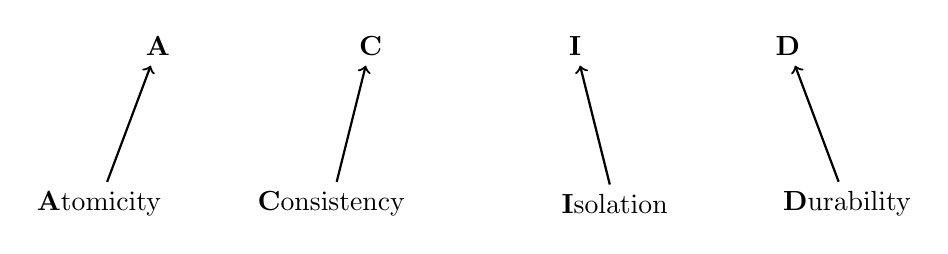
\begin{tikzpicture}[
    every node/.style={align=center},
    level distance=1.8cm
]

\node (A) at (-4,-2) {\textbf{A}};
\node (C) at (-1.3,-2) {\textbf{C}};
\node (I) at (1.3,-2) {\textbf{I}};
\node (D) at (4,-2) {\textbf{D}};

\node (A2) at (-4.75,-4) {\textbf{A}tomicity};
\node (C2) at (-1.8,-4) {\textbf{C}onsistency};
\node (I2) at (1.8,-4) {\textbf{I}solation};
\node (D2) at (4.75,-4) {\textbf{D}urability};




\draw[->, thick] (A2) to[] (A);
\draw[->, thick] (C2) to[] (C);
\draw[->, thick] (I2) to[] (I);
\draw[->, thick] (D2) to[] (D);

\end{tikzpicture}
\end{center}

\vspace{0.15cm}

\begin{center}
\begin{tikzpicture}[
    every node/.style={align=center},
    level distance=1.8cm
]

\node[draw, rectangle, minimum width=1cm, minimum height=3cm] (A) {};

\node[below=5mm of A] {Transaction};
\node[left=3cm of A] (B) {};
\node[right=3cm of A] (C) {};

\draw[->, shorten >=5pt] (B)-- node[midway, below] {Before\\(Coherent DB)} (A);
\draw[->,  shorten <=5pt] (A)-- node[midway, below] {After\\(Coherent DB)} (C);

\end{tikzpicture}
\end{center}

\vspace{0.25cm}
\section{Issue With Relational Data Base}
\begin{prettyBox}{Disponibility}{red}
    The constant \textbf{checking done to guarantee consistency} of data base after each transaction adds overhead which in turn \textbf{reduces the disponibility}.
\end{prettyBox}


\vspace{1cm}
\section{NoSQL Data Base Properties}

\vspace{.5cm}

\begin{center}
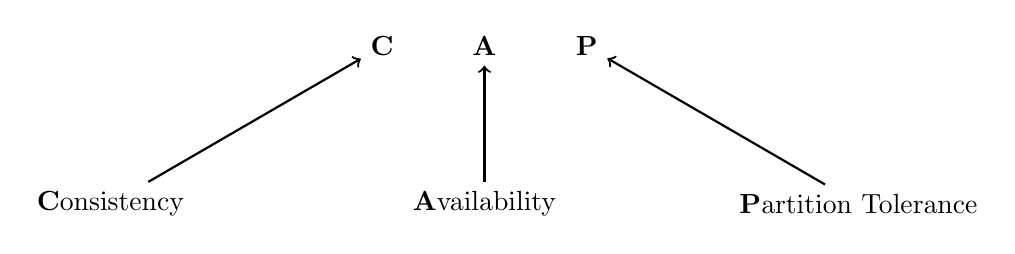
\begin{tikzpicture}[
    every node/.style={align=center},
    level distance=1.8cm
]

\node (C) at (-1.3,-2) {\textbf{C}};
\node (A) at (0,-2) {\textbf{A}};
\node (P) at (1.3,-2) {\textbf{P}};

\node (C2) at (-4.75,-4) {\textbf{C}onsistency};
\node (A2) at (0,-4) {\textbf{A}vailability};
\node (P2) at (4.75,-4) {\textbf{P}artition Tolerance};




\draw[->, thick] (C2) to[] (C);
\draw[->, thick] (A2) to[] (A);
\draw[->, thick] (P2) to[] (P);

\end{tikzpicture}
\end{center}



\end{document}

